\documentclass[aps,reprint,superscriptaddress,10pt]{revtex4-2}
\usepackage{kotex}
\usepackage[HWP]{dhucs-interword}
\usepackage[dvips]{color}
\usepackage{graphicx}
\usepackage{bm}
\usepackage{amsmath}
\usepackage{tikz}
\usepackage{mhchem}
\usepackage{booktabs}
\usepackage{multirow}
\usepackage{array}
\usepackage{tikz}

\begin{document}
\title{응집물질물리실험 결과보고서 \\
\small 실험주제 : Photo lithography}

\author{HuiJae-Lee}\email{hjlee6674@inha.edu}
\affiliation{Physics Department, Inha University}

\date{\today}


\begin{abstract}

 \end{abstract}
 
 \maketitle
 
\section{Process}

\section{Result}
\subsection{P-type}

\begin{figure}[htbp]
  \centering
  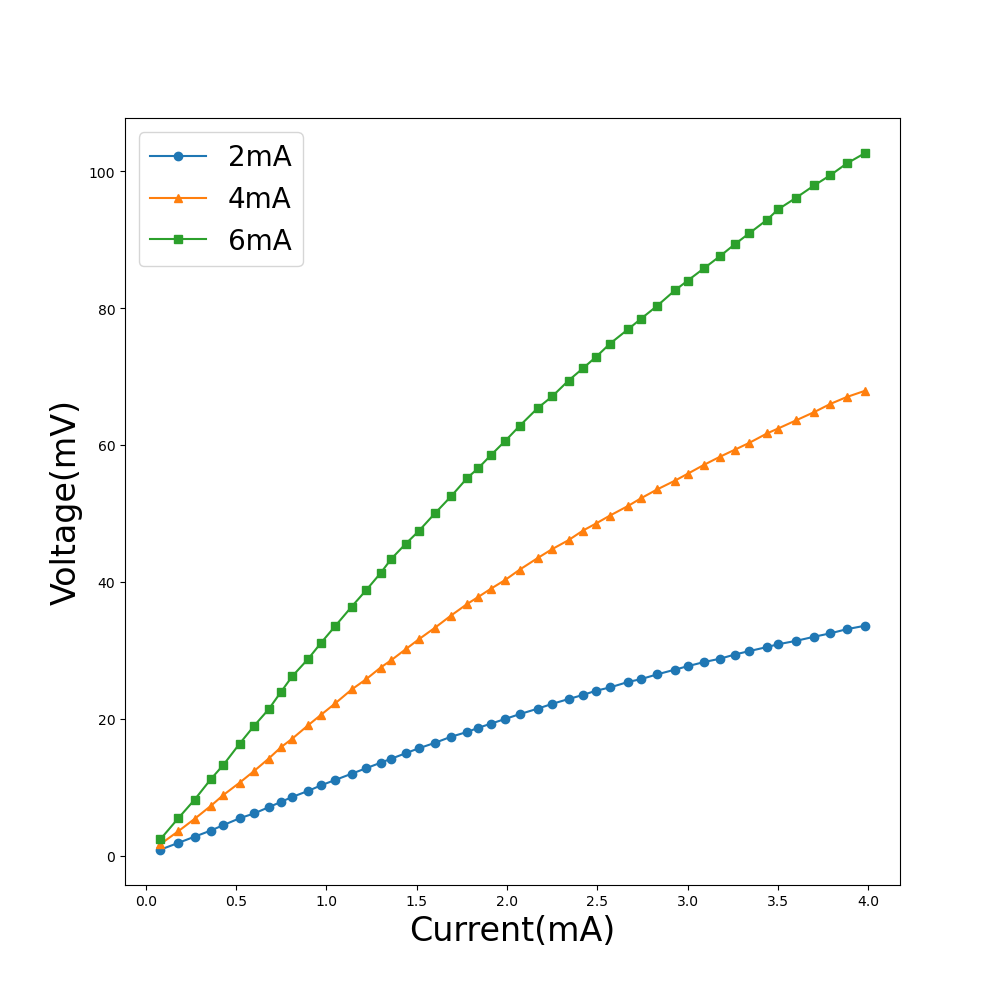
\includegraphics[scale = 0.15]{Hall_p.png}
  \caption{}
  \label{fig:p}
\end{figure}


\subsection{N-type}

\begin{figure}[htbp]
  \centering
  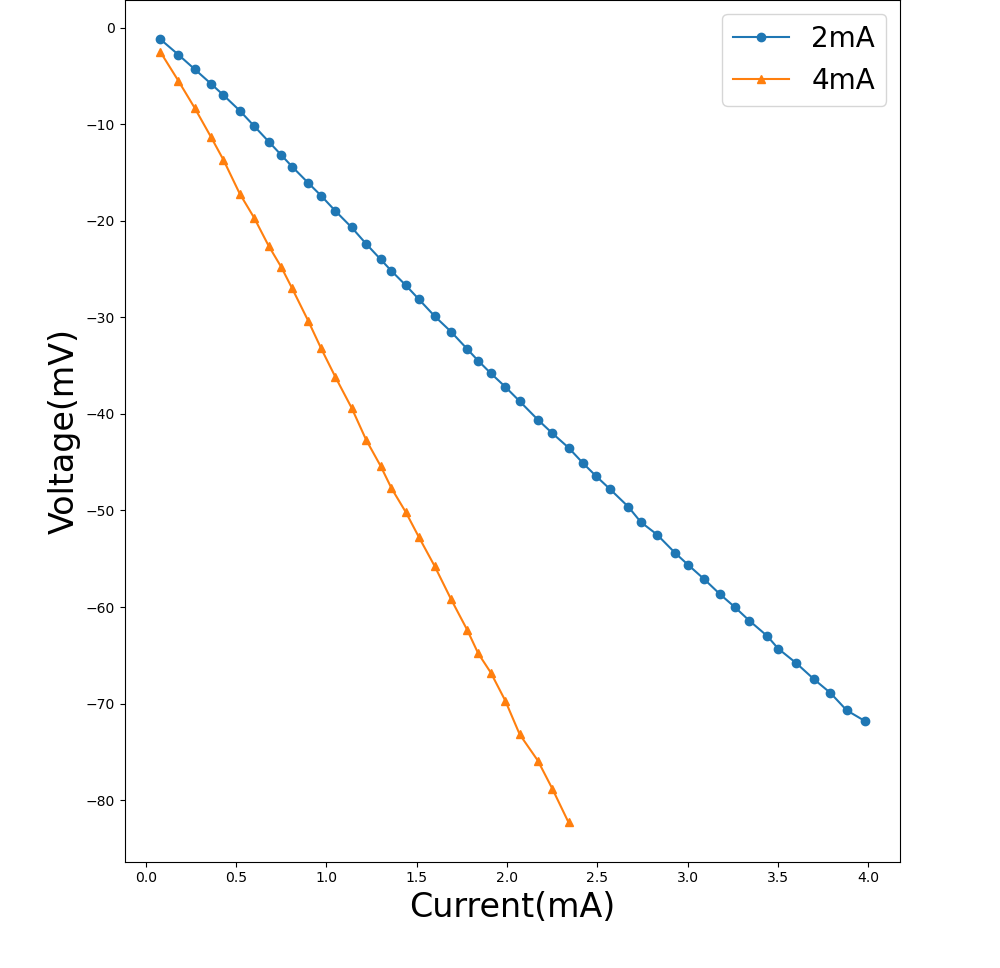
\includegraphics[scale = 0.15]{Hall_n.png}
  \caption{}
  \label{fig:p}
\end{figure}


\section{Conclusion}
  
  



\nocite{*} 
\bibliography{ref}



%\begin{thebibliography}{9}
%\end{thebibliography}

\vfill
\end{document}